\chapter{Implementierung}\label{ch:implementation}

\section{Anwendungsumgebung}\label{sec:implementation_environment}

Bevor die konkrete Implementierung der ausgewählten Contract-Testing-Frameworks erfolgen kann, ist ein Überblick über die zugrunde liegende Anwendungsumgebung notwendig.
Diese umfasst sowohl die technische Infrastruktur als auch die verwendeten Werkzeuge, Frameworks und Systemkomponenten, in welche die Contract-Tests eingebettet werden.
Ziel dieses Abschnitts ist es, die Rahmenbedingungen transparent darzustellen, unter denen die Integration und Ausführung der Tests erfolgt.
Dazu zählen insbesondere eingesetzte Programmiersprachen, Build- und Deployment-Pipelines, relevante Dienste sowie die Architektur der Kommunikationsbeziehungen zwischen Consumer und Provider.

Ein fundiertes Verständnis der Anwendungsumgebung ist essenziell, um die getroffenen Implementierungsentscheidungen nachvollziehbar zu machen und die spätere Übertragbarkeit der Ergebnisse auf andere Projekte realistisch einschätzen zu können.

Die Anwendung mit dem Namen \textit{msg.Sensorik} ist ein internes Projekt der msg systems ag, das als Grundlage für die Implementierung der Contract-Tests dient.
Sie dient ... % TODO: Zweck der Anwendung

Die Anwendung ist in einer Microservice-Architektur aufgebaut, wobei jeder Microservice eine spezifische Funktionalität bereitstellt und über jeweilige Schnittstellen kommuniziert.
Insgesamt ist die Anwendung in fünf verschiedene Microservices aufgeteilt:
\begin{itemize}
    \item \textbf{Instanz-Management-Service:} Dieser Service ist für die Erfassung und Verarbeitung von Stammdaten zuständig.
    \item \textbf{Regel-Service:} Er implementiert die Logik zur Verarbeitung von Sensordaten und zur Ausführung von Automatisierungsregeln.
    \item \textbf{Reporting-Service:} Dieser Service speichert den Verlauf von Sensordaten und stellt Berichte für die Visualisierung bereit.
    \item \textbf{Proxy-Service:} Der Proxy Service übernimmt die Kommunikation mit den Sensoren und Aktoren.
    \item \textbf{Nutzeroberfläche:} Die Nutzeroberfläche ermöglicht die Interaktion mit der Anwendung durch Benutzer.
\end{itemize}

Die technische Umsetzung der Anwendung basiert auf einem modernen Technologie-Stack, der für eine modulare und containerisierte Microservice-Architektur optimiert ist.

Die vier Backend-Services (Instanz-Management, Regel-Service, Reporting-Service und Proxy-Service) sind jeweils als eigenständige Spring-Boot-Anwendungen in Java realisiert und werden mit \gls{Maven} als Build-Tool verwaltet.
Diese bieten jeweils eine \gls{REST}-\gls{API} an, die von anderen Microservices konsumiert werden können.
Jeder dieser Services bringt seine eigene Datenhaltung mit, je nach Anwendungsfall entweder in Form von relationalen Datenbanken, \gls{NoSQL}-Datenbanken oder Zeitreihendatenbanken.
Die Nutzeroberfläche ist mit \gls{Angular} in TypeScript realisiert und greift über \gls{REST}-\glspl{API} auf die Backend-Services zu.

Die Microservices interagieren untereinander sowohl als Consumer als auch als Provider.
Beispielsweise konsumiert der Proxy-Service Daten vom Blablabla-Service, fungiert aber auch als Provider, während die Nutzeroberfläche lediglich als Consumer auftritt und \zB die Stammdaten vom Instanz-Management-Service anfragt.
Eine Consumer/Provider-Matrix ist in \cref{tab:consumer_provider_matrix} dargestellt, um die Kommunikationsbeziehungen zwischen den einzelnen Microservices zu veranschaulichen.
Diese Kommunikationsbeziehungen bilden die Grundlage für die Definition der Contracts in \cref{sec:implementation_execution}.

\begin{table}[htbp]
    \centering
    \vspace{1ex}
    \begin{tabular}{@{}l|ll@{}}
        \toprule
        Service            & Provider & Consumer \\
        \midrule
        Instanz-Management & Ja       & Ja       \\
        Regel              & Ja       & Nein     \\
        Reporting          & Ja       & Nein     \\
        Proxy              & Ja       & Ja       \\
        Nutzeroberfläche   & Nein     & Ja       \\
        \bottomrule
    \end{tabular}
    \vspace{2ex}
    \caption{Consumer/Provider-Matrix der Microservices}
    \label{tab:consumer_provider_matrix}
\end{table}

Die Containerisierung der Service-Bausteine erfolgt mithilfe von \texttt{Docker}, wobei die einzelnen Anwendungsumgebungen über \texttt{docker-compose} orchestriert werden.
Dadurch lässt sich eine konsistente und reproduzierbare Ausführungsumgebung gewährleisten.

Für Versionsverwaltung und Repositories kommt eine zentral vom Unternehmen gehostete \texttt{Gitea}-Instanz zum Einsatz.
Jeder Microservice befindet sich in einem eigenen Git-Repository, was eine getrennte Entwicklung und Versionierung erlaubt.

Die Continuous Integration erfolgt über \texttt{Drone CI}, das eng mit \texttt{Gitea} integriert ist.
Die Pipeline-Schritte umfassen unter anderem das Ausführen von Unit- und Integrationstests, das Bauen und Versionieren der Anwendung sowie die Überprüfung der Code-Qualität und Sicherheitsstandards durch statische Code-Analyse mit dem Tool \texttt{SonarQube}.
Genau wie Gitea sind auch \texttt{Drone CI} und \texttt{SonarQube} in der Infrastruktur des Unternehmens gehostet.

\section{Technische Umsetzung}\label{sec:implementation_execution}

Die Umsetzung der Contract-Tests erfolgte iterativ in einer lokalen Entwicklungsumgebung, um eine möglichst isolierte und kontrollierte Integration der einzelnen Frameworks zu gewährleisten.
Zunächst musste die lokale Testumgebung der Microservice-Anwendung vorbereitet werden, um die Contract-Tests ausführen zu können.
Ein zentrales Element der Implementierung war die Einrichtung eines lokalen \texttt{Pact Broker}, der als zentrales Austauschsystem zwischen Consumer- und Provider-Services dient.
Der Broker wurde in einem Docker-Container betrieben, um eine einfache Handhabung und Portabilität zu gewährleisten.

\subsection{Consumer-Contract als Ausgangspunkt}\label{subsec:implementation_execution_consumer-contract}

Getreu nach den \gls{CDCT}-Prinzipien erfolgte der Einstieg in die Contract-Test-Implementierung beim Service der Nutzeroberfläche, welcher als Consumer einiger Backend-\glspl{API} fungiert.
Zuerst musste eines der Plugins für \texttt{Pact} ausgewählt werden, welches Consumer-Tests in \texttt{TypeScript} unterstützt.
Die Wahl fiel letztendlich auf \texttt{pact-js}, welches von der offiziellen Pact empfohlen wird~\cite{pactfoundationPactDocs2022}.
Weitere Ausführungen dazu finden sich in \cref{subsec:implementation_problems_angular-integration}.
Damit wurden die Tests im Nutzeroberflächen-Service-Repository in einem separaten Verzeichnis als die Angular-Anwendung in TypeScript formuliert, da die Angular-Anwendung Probleme mit Abhängigkeiten der \texttt{pact-js}-Bibliothek hatte.
Nähere Informationen der Herausforderung der Einrichtung von Contract-Tests in Angular sind in \cref{sec:implementation_problems} zu finden.

Für die Erstellung der Testfälle wurde sich an den Methoden der Service-Klassen der Angular-Anwendung orientiert, da diese die tatsächlichen Interaktionen mit den Backend-Services im Code abbilden.
Für jede der genutzten HTTP-Verben (GET, POST, PUT, DELETE) der einzelnen \gls{API}-Pade wurde ein separater Consumer-Test definiert, der die erwarteten Interaktionen mit dem zugehörigen Provider-Service beschreibt.
Als Erstes wurde für jede Interaktion ein Status definiert, der beschreibt, in welchem Status sich der Provider zur Zeit der Provider-Verifizierung befinden muss, um die zugehörige Antwort zurückliefern zu können.
Danach wird die Anfrage festgelegt, die der Consumer an den Provider sendet, einschließlich der HTTP-Methode, des Pfads, der Header und der Payload.
Die erwartete Antwort des Providers wird ebenfalls spezifiziert, einschließlich des HTTP-Statuscodes und der erwarteten Antwortdaten.
Dabei können auch komplexe Datenstrukturen und Validierungsregeln der Antwortinhalte definiert werden, um sich ändernde Werte zu berücksichtigen.
Diese Angaben dienen als Grundlage für den Provider-Mock, gegen den die Aufrufe der Angular-Anwendung getestet werden.

Außerdem werden Erwartungen definiert, die bei der Ausführung der Consumer-Tests gegen den Provider-Mock erfüllt sein müssen, um die simulierte Interaktion zu überprüfen.
So kann sichergestellt werden, dass die Angular-Anwendung die erwarteten Antworten korrekt verarbeitet.
Nach erfolgreicher Ausführung der Consumer-Tests wird ein Pact-Contract generiert, der diese definierten Interaktionen zwischen Consumer und Provider beschreibt und als JSON-Datei speichert.
Ein Beispiel für einen solchen Pact-Contract ist in \cref{lst:pact_contract_example} zu finden.

\lstinputlisting[language=JSON, caption=Beispiel für einen Pact-Contract, label=lst:pact_contract_example]{listings/example-contract.json}

Zur Ausführung der Tests kam das Test-Framework \texttt{Jasmine} zum Einsatz, welches in dieser Angular-Anwendung bereits für andere Testarten verwendet wird.
Nach erfolgreicher Definition und Ausführung der Consumer-Tests wurde der erstellte Pact-Contract unter Angabe der Service-Version über die Pact CLI an den \texttt{Pact Broker} publiziert.

\subsection{Provider-Verifizierung}\label{subsec:implementation_execution_provider-verification}

Im Anschluss wurde der zugehörige Provider-Test aufseiten des Instanz-Management-Service implementiert.
Die Verifizierung der Consumer-Verträge erfolgte mit \texttt{Junit5} und dem \texttt{pact-jvm}-Provider-Framework.
Dazu wurde die entsprechende Abhängigkeit mithilfe von \gls{Maven} in das Projekt eingebunden und Konfigurationen wie Eintragen der Broker-URL durchgeführt.
Dieses Framework ermöglicht es, die im Pact-Contract definierten Interaktionen gegen die tatsächliche Implementierung des Providers automatisiert zu prüfen.
Es musste lediglich eine Testklasse mit einem \texttt{TestTemplate} erstellt werden, die die Consumer-Interaktionen aus dem Pact-Contract lädt und gegen die Provider-Implementierung validiert.
Um die erwarteten Zustände für die Vertragsprüfung zu simulieren (\zB vorhandene Entitäten in der Datenbank), wurden sogenannte \texttt{State Definitions} im Provider eingerichtet.
Dazu musste für jeden Zustand eine Status-Methode definiert werden, die den Provider in den erwarteten Zustand versetzt, bevor der entsprechende Test ausgeführt wird.
Nach erfolgreicher Durchführung der Provider-Tests wird der Contracts im \texttt{Pact Broker} automatisch als verifiziert, markiert und Services, die mit diesem Contract kompatibel sind, können deployt werden.

Nach erfolgreicher Implementierung der Contract-Tests für die Kommunikation der Nutzeroberfläche mit dem Instanz-Management-Service wurde der Prozess sukzessive für die anderen Microservices wiederholt, wobei nun die Consumer-Seite auch mit dem \texttt{pact-jvm}-Framework implementiert werden musste.
Diese Durchführung erfolgte nach demselben Muster wie bei der Nutzeroberfläche, wobei jedoch die Syntax und die spezifischen Implementierungsdetails durch die verwendete Programmiersprache Java abwichen.
Für die Veröffentlichung der Contracts musste noch das CLI-Plugin über \texttt{Maven} installiert werden, um die Pact-Contracts an den \texttt{Pact Broker} zu übermitteln.

Jede Service-Interaktion durchlief dabei denselben Zyklus: Definition der Consumer-Seite, Veröffentlichung zum Pact Broker, Implementation und Ausführung des Provider-Tests, Veröffentlichung des Verifizierungsstatus.
Die Contract-Tests wurden für alle relevanten Interaktionen zwischen den Microservices implementiert, um die Interoperabilität und Konsistenz der Kommunikation sicherzustellen.
Dabei sind insgesamt sechs Contracts zwischen den fünf Microservices entstanden, die die Interaktionen zwischen den Services abbilden.
Diese sind mithilfe eines Abhängigkeitsgraphen in \cref{fig:service_dependecies} visualisiert, welcher durch den \texttt{Pact Broker} automatisch generiert wurde.

\begin{figure}[htbp]
    \centering
    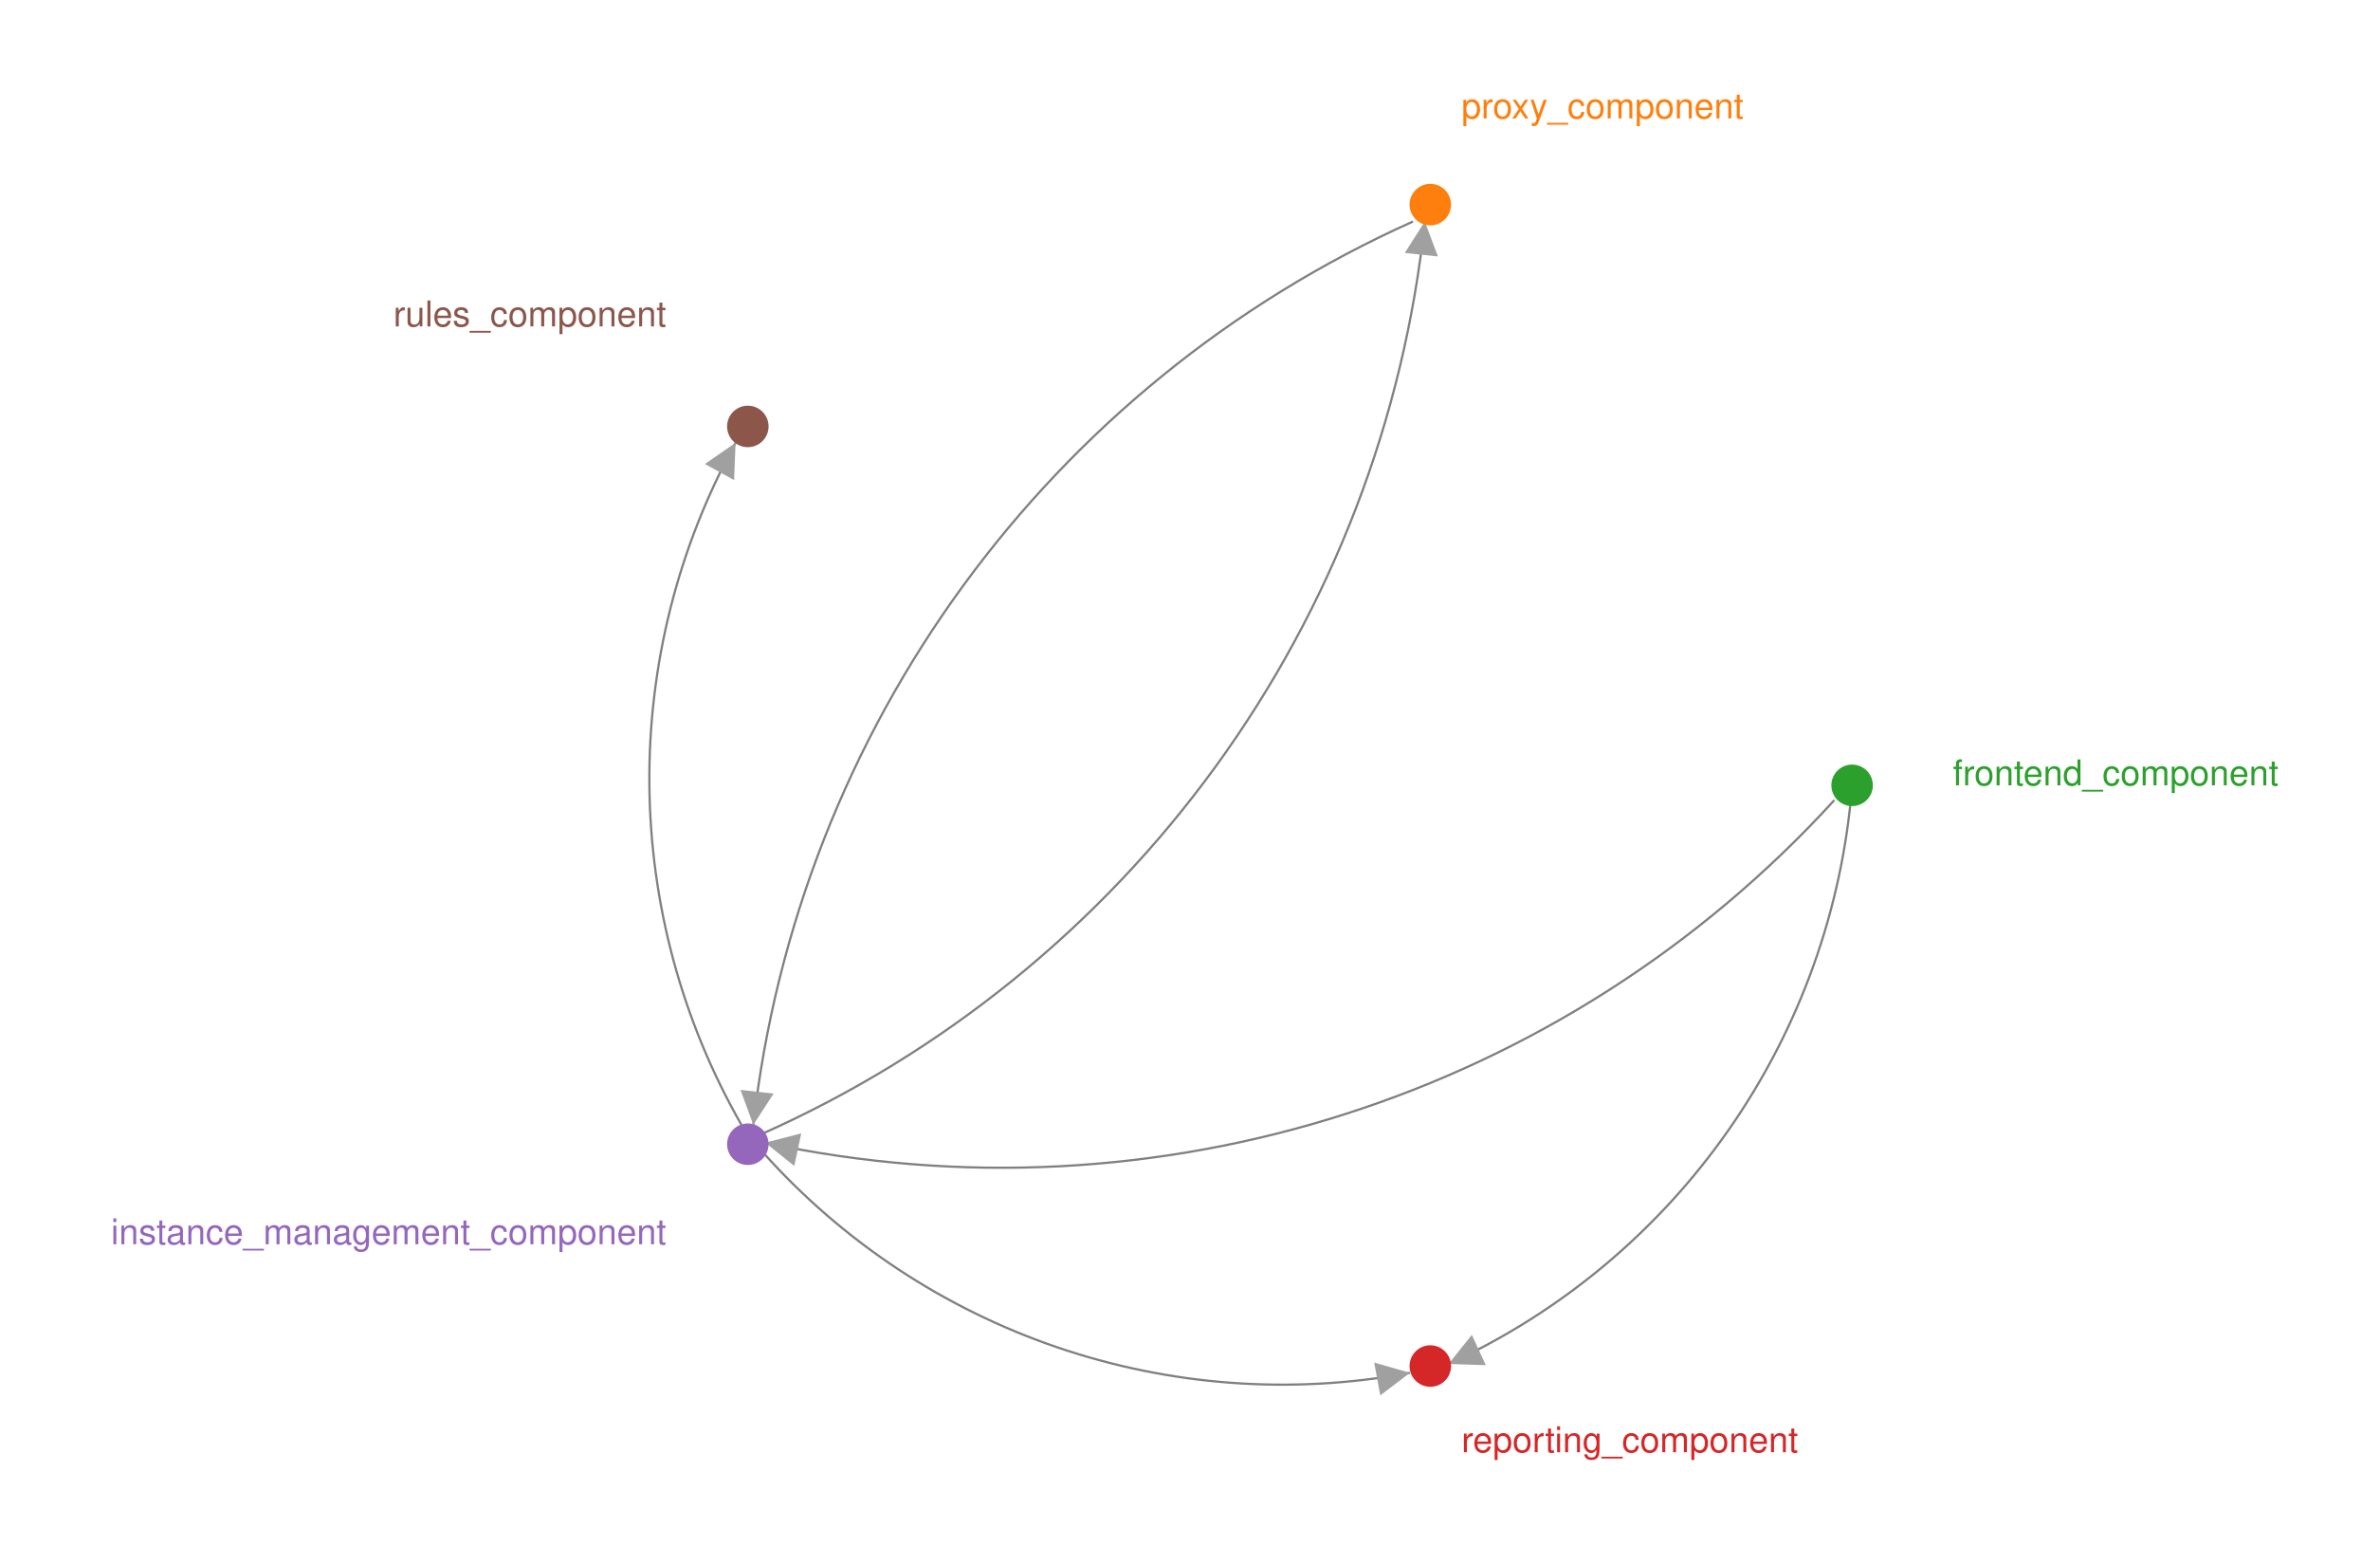
\includegraphics[width=0.8\textwidth]{figures/service-dependencies}
    \caption{Abhängigkeitsgraph der Microservices}
    \label{fig:service_dependecies}
\end{figure}

\subsection{CI-Integration und Automatisierung}\label{subsec:implementation_execution_ci-integration}

Um die vollständige \gls{CI}/\gls{CD}-Pipeline auch abbilden zu können, musste zusätzlich ein lokales \texttt{Drone CI}-System aufgesetzt und mit dem \texttt{Pact Broker} verbunden.
Eine Durchführung der Contract-Tests in der lokalen Umgebung war notwendig, da die zentrale \texttt{Drone CI}-Instanz des Unternehmens aus netzwerktechnischen Gründen nicht ohne Weiteres mit einem lokalen \texttt{Pact Broker} verbunden werden kann.
Mit dieser lokalen \texttt{Drone CI}-Instanz konnte für jeden Microservice eine Pipeline konfiguriert werden, die die Contract-Tests automatisch ausführt und deren Ergebnisse im \texttt{Pact Broker} speichert.
Die Pipeline umfasst je nach Service die Schritte:
\begin{itemize}
    \item Ausführen der Consumer-Tests, um den Pact-Contract zu generieren.
    \item Publizieren des Pact-Contracts an den \texttt{Pact Broker}.
    \item Ausführen der Provider-Verifizierungstests gegen den Pact-Contract.
    \item Aktualisieren des Verifizierungsstatus im \texttt{Pact Broker}.
    \item Can-I-Deploy-Abfrage an den \texttt{Pact Broker}, um zu prüfen, ob der Service mit den aktuellen Contracts kompatibel ist.
\end{itemize}

Die Automatisierung dieser Schritte ermöglicht eine nahtlose Integration der Contract-Tests in den Entwicklungsprozess und stellt sicher, dass Änderungen an den Services sofort auf ihre Interoperabilität geprüft werden.

\section{Probleme und Herausforderungen}\label{sec:implementation_problems}

Die Einführung von Contract-Tests im Projektumfeld brachte eine Reihe technischer und konzeptioneller Herausforderungen mit sich, wie schon in \cref{sec:implementation_execution} angedeutet, die im Verlauf der Implementierung identifiziert und schrittweise gelöst wurden.
Die folgenden Abschnitte skizzieren die zentralen Problemfelder und beschreiben, wie diesen begegnet wurde.

\subsection{\gls{CI}-Infrastrukturkomplexität}\label{subsec:implementation_problems_ci-infrastructure}

Ein zentrales Hindernis zu Beginn der Umsetzung war die Einrichtung einer funktionsfähigen lokalen Testumgebung, die alle beteiligten Komponenten – insbesondere den \texttt{Pact Broker} und das CI-System \texttt{Drone CI} und die Versionsverwaltung \texttt{Gitea} – umfasst.
Beide Dienste mussten in einer Weise konfiguriert werden, dass die vollständige Kommunikationskette zwischen Consumer-Tests, Pact-Veröffentlichung und Provider-Verifikation ohne manuelle Zwischenschritte möglich war.

Da für die prototypische Implementierung keine zentrale \texttt{Pact Broker}-Instanz zur Verfügung stand, musste eine lokale Instanz aufgesetzt werden.
Um die Integration in die \texttt{Drone CI}-Pipeline zu ermöglichen, musste auch die \texttt{Drone CI}-Instanz lokal betrieben werden, da die zentrale \texttt{Drone CI}-Instanz des Unternehmens nicht auf den lokalen \texttt{Pact Broker} zugreifen kann.
Ein Server kann nicht direkt auf einen lokalen Rechner zugreifen, da dies durch grundlegende Prinzipien der Netzwerksicherheit und -architektur verhindert wird.
Lokale Rechner befinden sich meist hinter Firewalls und nutzen private IP-Adressen, die durch Network Address Translation vom öffentlichen Internet abgeschirmt sind~\cite{moskowitzAddressAllocationPrivate1996}.

Bei der Verbindung der zentralen \texttt{Gitea}-Instanz mit der lokalen \texttt{Drone CI}-Instanz traten ebenfalls Schwierigkeiten auf.
Die meisten Interaktionen zwischen \texttt{Gitea} und \texttt{Drone CI} gehen von der \gls{CI}-Pipeline aus, die auf \texttt{Gitea} zugreift, um Repository zu klonen und so den aktuellen Stand des Codes zu erhalten.
Allerdings erfolgt die Benachrichtigung der \texttt{Drone CI}-Instanz über neue Commits oder Pull-Requests mittels Webhooks von \texttt{Gitea} aus~\cite{DroneCICD}, was in diesem Fall nicht möglich war, da die lokale \texttt{Drone CI}-Instanz nicht von \texttt{Gitea} erreicht werden konnte.
So konnten die Pipelines nicht automatisch ausgelöst werden und mussten manuell gestartet werden, was die Aussage der prototypischen Implementierung aber nicht beeinträchtigt.
Eine ebenfalls manuelle Installation einer \texttt{Gitea}-Instanz wäre zwar möglich gewesen, aber nicht zielführend, da das eine erhebliche Umstellung der Infrastruktur und Redundanz bedeutet hätte.

\subsection{Angular-Integration}\label{subsec:implementation_problems_angular-integration}

Die Integration der Contract-Tests in die Angular-Anwendung stellte eine besondere Herausforderung dar, da die Angular-Entwicklungsumgebung und die verwendeten Abhängigkeiten nicht optimal mit den \texttt{pact-js}-Bibliotheken harmonierten.

Viele Anleitungen und Beispiele für den \texttt{Angular}-Context beziehen sich auf die Kombination von den \texttt{pact-web}, \texttt{pact-node} \bzw \texttt{karma-pact} Plugin~\cite{hendricksenConsumerDrivenContractTesting2020, hombergsCreatingConsumerDrivenContract2017}, welche jedoch nicht mehr verwendet werden sollten, da sie nicht mehr aktiv gepflegt werden~\cite{PactfoundationPactweb2022, PactfoundationKarmapactPact}.
Deshalb wurde auf die Implementierung mithilfe von \texttt{pact-js} gesetzt, welches die Consumer-Tests in TypeScript unterstützt und von der Pact Foundation empfohlen wird~\cite{pactfoundationPactDocs2022}.

Bei der Integration von \texttt{pact-js} in die Angular-Anwendung traten aber Abhängigkeitskonflikte auf, die eine direkte Verwendung der Bibliothek in der Angular-Umgebung verhinderten.
Da die direkte Integration in die Angular-Anwendung nicht nötig war, wurde stattdessen ein separates Verzeichnis innerhalb des Repositories erstellt, in dem die Consumer-Tests unabhängig von der Angular-Anwendung ausgeführt werden konnten.
Dort musste allerdings eine neue Node.js-Umgebung eingerichtet werden, die die Abhängigkeiten für \texttt{pact-js}, \texttt{Jasmine} \usw verwaltet.

\subsection{Provider-Verifizierung}\label{subsec:implementation_problems_provider-verification}

Auch bei der Implementierung der Provider-Verifizierungstests trat eine kleine Herausforderung auf, wodurch die Tests nicht direkt gegen die reale Implementierung des Providers ausgeführt wurden.
Die im Contract definierten Requests wurden am Anfang an einen zufälligen Port gesendet, der nicht mit dem Port des laufenden Providers übereinstimmte.
Dies führte dazu, dass die Tests fehlschlugen, da auf dem angesprochenen Port nicht die erwartete Antwort zurückgegeben wurde.
Da aber auf diesem Port ein anderer undefinierter Server lief und mit HTTP-Responses antwortete, wurde der Fehler nicht als dieser sofort erkannt.

Die Lösung bestand darin, den Port des Providers in der Testkonfiguration explizit anzugeben, sodass die Anfragen an den richtigen Port gesendet wurden.
Es wurde eine Konfiguration in der Testklasse erstellt, die den Port des laufenden Providers ermittelt und für die Tests als Zielport spezifiziert.